\documentclass{article}[18pt]
\ProvidesPackage{format}
%Page setup
\usepackage[utf8]{inputenc}
\usepackage[margin=0.7in]{geometry}
\usepackage{parselines} 
\usepackage[english]{babel}
\usepackage{fancyhdr}
\usepackage{titlesec}
\hyphenpenalty=10000

\pagestyle{fancy}
\fancyhf{}
\rhead{Sam Robbins}
\rfoot{Page \thepage}

%Characters
\usepackage{amsmath}
\usepackage{amssymb}
\usepackage{gensymb}
\newcommand{\R}{\mathbb{R}}

%Diagrams
\usepackage{pgfplots}
\usepackage{graphicx}
\usepackage{tabularx}
\usepackage{relsize}
\pgfplotsset{width=10cm,compat=1.9}
\usepackage{float}

%Length Setting
\titlespacing\section{0pt}{14pt plus 4pt minus 2pt}{0pt plus 2pt minus 2pt}
\newlength\tindent
\setlength{\tindent}{\parindent}
\setlength{\parindent}{0pt}
\renewcommand{\indent}{\hspace*{\tindent}}

%Programming Font
\usepackage{courier}
\usepackage{listings}
\usepackage{pxfonts}

%Lists
\usepackage{enumerate}
\usepackage{enumitem}

% Networks Macro
\usepackage{tikz}


% Commands for files converted using pandoc
\providecommand{\tightlist}{%
	\setlength{\itemsep}{0pt}\setlength{\parskip}{0pt}}
\usepackage{hyperref}

% Get nice commands for floor and ceil
\usepackage{mathtools}
\DeclarePairedDelimiter{\ceil}{\lceil}{\rceil}
\DeclarePairedDelimiter{\floor}{\lfloor}{\rfloor}

% Allow itemize to go up to 20 levels deep (just change the number if you need more you madman)
\usepackage{enumitem}
\setlistdepth{20}
\renewlist{itemize}{itemize}{20}

% initially, use dots for all levels
\setlist[itemize]{label=$\cdot$}

% customize the first 3 levels
\setlist[itemize,1]{label=\textbullet}
\setlist[itemize,2]{label=--}
\setlist[itemize,3]{label=*}

% Definition and Important Stuff
% Important stuff
\usepackage[framemethod=TikZ]{mdframed}

\newcounter{theo}[section]\setcounter{theo}{0}
\renewcommand{\thetheo}{\arabic{section}.\arabic{theo}}
\newenvironment{important}[1][]{%
	\refstepcounter{theo}%
	\ifstrempty{#1}%
	{\mdfsetup{%
			frametitle={%
				\tikz[baseline=(current bounding box.east),outer sep=0pt]
				\node[anchor=east,rectangle,fill=red!50]
				{\strut Important};}}
	}%
	{\mdfsetup{%
			frametitle={%
				\tikz[baseline=(current bounding box.east),outer sep=0pt]
				\node[anchor=east,rectangle,fill=red!50]
				{\strut Important:~#1};}}%
	}%
	\mdfsetup{innertopmargin=10pt,linecolor=red!50,%
		linewidth=2pt,topline=true,%
		frametitleaboveskip=\dimexpr-\ht\strutbox\relax
	}
	\begin{mdframed}[]\relax%
		\centering
		}{\end{mdframed}}



\newcounter{lem}[section]\setcounter{lem}{0}
\renewcommand{\thelem}{\arabic{section}.\arabic{lem}}
\newenvironment{defin}[1][]{%
	\refstepcounter{lem}%
	\ifstrempty{#1}%
	{\mdfsetup{%
			frametitle={%
				\tikz[baseline=(current bounding box.east),outer sep=0pt]
				\node[anchor=east,rectangle,fill=blue!20]
				{\strut Definition};}}
	}%
	{\mdfsetup{%
			frametitle={%
				\tikz[baseline=(current bounding box.east),outer sep=0pt]
				\node[anchor=east,rectangle,fill=blue!20]
				{\strut Definition:~#1};}}%
	}%
	\mdfsetup{innertopmargin=10pt,linecolor=blue!20,%
		linewidth=2pt,topline=true,%
		frametitleaboveskip=\dimexpr-\ht\strutbox\relax
	}
	\begin{mdframed}[]\relax%
		\centering
		}{\end{mdframed}}
\lhead{Software Methodologies - Computer Graphics}


\begin{document}
\begin{center}
\underline{\huge Graphics Pipeline for Interactive Rendering}
\end{center}
\section{Rendering in Computer Graphics}
Rendering pipeline comprises of operations converting 3D geometry into a 2D pixel representation for display\\
\\
Two types:
\begin{itemize}
	\item Fixed Function - Use a standard set of operations to efficiently generate pixel representation from 3D polygons based on their visibility
	\item Programmable - Focus on the flexibility in programming and the utilisation of the parallel processing capability of the GPU
\end{itemize}
Fixed Function Pipeline
\begin{center}
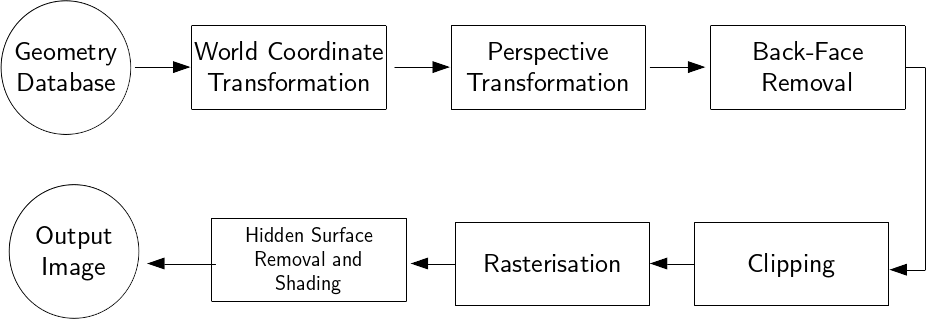
\includegraphics[scale=0.6]{Fixed-Function}
\end{center}
Programmable Rendering Pipeline
\begin{center}
	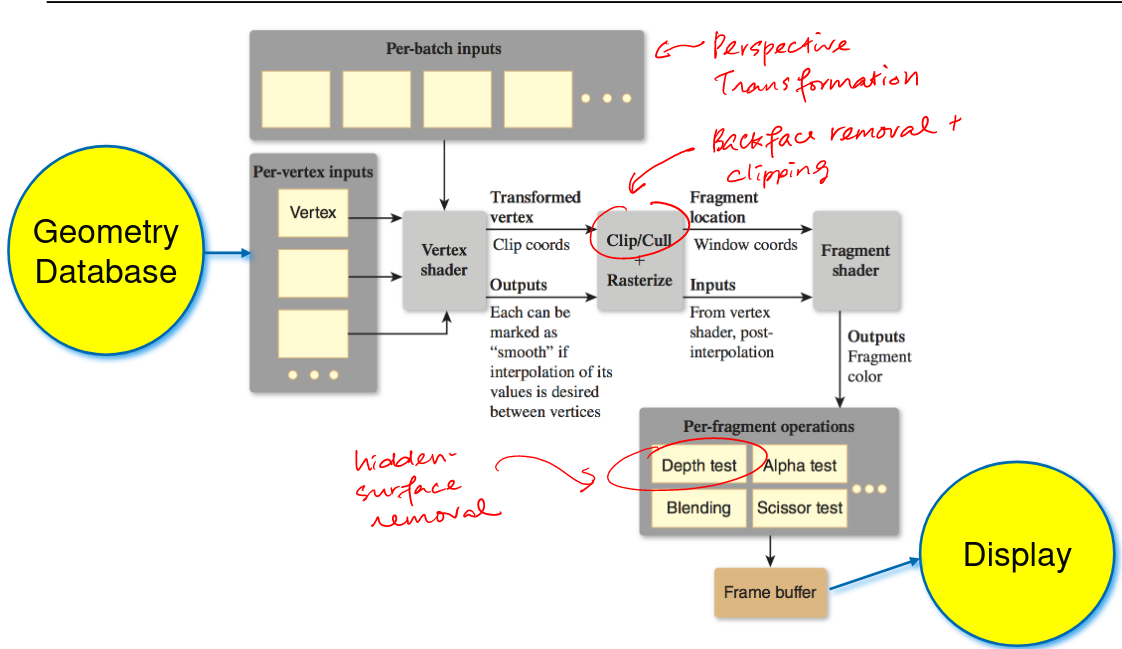
\includegraphics[scale=0.4]{programmable}
\end{center}
\section{Local and World Coordinate}
\begin{itemize}
	\item \textbf{Geometry Database} - Each object in the scene is first created using a software program in its local coordinate system
	\item \textbf{World coordinate transformation} - Transforms each object to a common world coordinate system
\end{itemize}
\section{Back Face Removal}
Remove surfaces of a solid object which are facing away from the viewer. They may contribute to approximately half of the total number of surfacers in a scene
\begin{definition}[Front Faces]
Object surface facing the viewer
\end{definition}
\begin{definition}[Back faces]
Object surface facing away from the viewer
\end{definition}
\section{Clipping}
Clipping is a process to determine the portion of an object lying inside (or outside) a region called the clip region
\begin{definition}[Clip region]
Typically either a window on a screen or a view volume
\end{definition}
The Cohen-Sutherland Line-Clipping Algorithm works by dividing the area around the clip region as follows
\begin{center}
	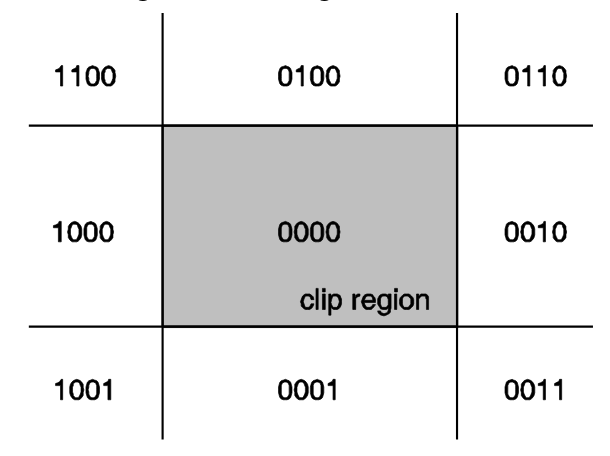
\includegraphics[scale=0.7]{Clipping}
\end{center}
\begin{itemize}
	\item This allows us to quickly identify lines to be trivially accept/reject
	\item If both ends of the line are in the clip region then the line can be accepted
	\item If two of the code words of a line have the same bit set to 1, the line is completely outside and can be rejected
	\item Otherwise, the line needs to be clipped
\end{itemize}
\section{Rasterization}
Break a primitive into pixel fragments
\begin{center}
	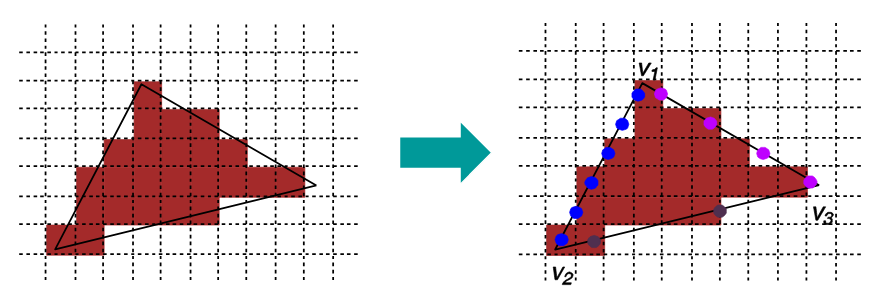
\includegraphics[scale=0.7]{Rasterization}
\end{center}
\begin{itemize}
	\item Consider rasterizing a triangle $(v_1,v_2,v_3)$
	\item Interpolate $v_1$ and $v_2$ to produce an interpolated point for each row of pixels between $v_1$ and $v_2$
	\item We do the same for $v_1$ and $v_3$ as well as $v_3$ and $v_2$
	\item Each pair of interpolated points on a row is called a scanline
	\item We then interpolate between the pair of interpolated points to form pixel fragments
	\item Interpolate along the primitive edges followed by the interior pixels between pairs of interpolated points (scanlines)
	\item Such interpolation is referred to as bilinear interpolation
\end{itemize}
\section{Primitive Drawing on a 2D screen}
Painter's algorithm
\begin{itemize}
	\item Paint distance parts of a scene before parts which are nearer to users, however this can have ambiguity
\end{itemize}
\subsection{Z-Buffering}
The most popular hidden surface removal method is the z-buffer method, which is implemented by the majority of existing graphics accelerators\\
\\
The z-buffer method requires two buffers:
\begin{itemize}
	\item z-buffer (or depth buffer): determine the nearest primitive fragment at each screen pixel
	\item image buffer: store the colour value of the nearest primitive fragment at each pixel
\end{itemize}
Finally, the shading step computes the colour of each visible primitive at each pixel location based on some shading methods
\section{Specular lighting}
\begin{itemize}
	\item Bright spot on the object
	\item Resultant reflection of the incident light concentrates in a local region
\end{itemize}
Calculation
$$\text{Specular Lighting } = K_s\times I \times \cos^n(\phi)$$
$K_s$ - Specular reflection coefficient\\
$N$: surface normal at P\\
$I$: light intensity\\
$\phi$: angle between V and R\\
$\cos^n(\phi)$ - The large the value of N, the smaller the cos value
\begin{center}
	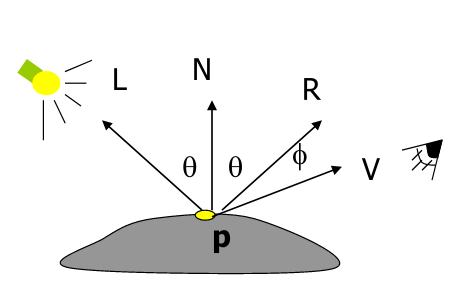
\includegraphics[scale=0.7]{Specular_Lighting}
\end{center}

\end{document}